\documentclass[11pt, a4paper, twoside, reqno]{article}
\usepackage[utf8]{inputenc}
\usepackage[cm]{fullpage}
\usepackage{amssymb}
\usepackage{graphics}
\usepackage{graphicx}
\usepackage{amsmath}
\usepackage{amscd}
\usepackage{amsthm}
\usepackage{mathrsfs}
\usepackage{amsfonts}
\usepackage{lscape}
\usepackage{float}
\usepackage{lineno,hyperref}
\hypersetup{hidelinks}
\usepackage{orcidlink}
\usepackage{caption}
\usepackage[colorinlistoftodos]{todonotes}
\usepackage[linesnumbered,boxed,lined,ruled,vlined]{algorithm2e}
\usepackage{natbib}
\usepackage[left=2.5cm, right=2.5cm, top=2cm, bottom=3cm]{geometry}
\modulolinenumbers[5]
\thispagestyle{plain}
\usepackage{fancyhdr}
\fancypagestyle{mypagestyle}{%
  \fancyhf{}%
  \fancyhead[OC]{\footnotesize{A. HUSEYNLI et al.: TABLE PLACEMENT AND TIMING LEAKAGE IN DIPPER}}%
  \fancyhead[EC]{\footnotesize{JOURNAL OF MODERN TECHNOLOGY AND ENGINEERING, V.XX, N.XX, 20XX}}%
  \fancyfoot[C]{\thepage}%
  \renewcommand{\headrulewidth}{1.2pt}%
  \setlength{\headheight}{12.2pt}
  \setlength{\headsep}{15pt}
  \renewcommand{\headrulewidth}{0.8pt}
} \pagestyle{mypagestyle} \setcounter{page}{1}

% no stretched vertical space between paragraphs and headings (twoside sets \flushbottom)
\raggedbottom
% let floats fill pages normally
\renewcommand{\topfraction}{0.9}
\renewcommand{\bottomfraction}{0.8}
\renewcommand{\textfraction}{0.1}
\renewcommand{\floatpagefraction}{0.8}

\newtheorem{theorem}{Theorem}
\newtheorem{definition}{Definition}
\newtheorem{remark}{Remark}

\newcommand{\tsm}{\texttt{small}}
\newcommand{\tfa}{\texttt{fast}}
\newcommand{\tfc}{\texttt{fast\_const}}
\newcommand{\tct}{\texttt{ct}}
\newcommand{\tlk}{\texttt{leaky}}

\begin{document}
\vspace{-2.5cm} \hrule \vspace{0.15cm}
\hfill{\scalebox{0.5}{
\includegraphics[]{logo.eps}}}

\vspace{-1.1cm} \noindent {\small Journal of Modern Technology and Engineering}\\
\noindent {\small Vol.XX, No.XX, 20XX, pp.xx--xx} \vspace{0.18cm}
\hrule \vspace{1.5cm}

\noindent {\large \bf TABLE PLACEMENT AND TIMING LEAKAGE IN DIPPER IMPLEMENTATIONS}

\vspace*{6mm}

\noindent{\bf \orcidlink{0009-0003-4959-2887}\,Ali Huseynli$^{1*}$, \orcidlink{0000-0002-3710-1046}\,Yadigar Imamverdiyev$^{1}$, \orcidlink{0009-0003-6410-3711}\,Jalal Alizadeh$^{1}$}\\
\noindent{$^{1}$Azerbaijan Technical University, Baku, Azerbaijan}\\

\hrule \vspace{0.2cm} \noindent {\footnotesize{\bf Abstract.}
Secret-indexed table lookups are a classic source of timing leakage, but whether they leak depends on the memory path between the core and the table. We test five C implementations of the Dipper-64/128 lightweight block cipher on ten hardware platforms, from Cortex-M microcontrollers to an x86-64 server, with a dudect-style fixed-versus-random Welch $t$-test computed on the device and a rule that every leak must repeat in an independent run. Tables read from flash leak on four microcontrollers, while the same tables in RAM do not. A controlled experiment, in which identical code reads identical tables from RAM or from flash, confirms that placement alone decides. On three of these chips a lookup-latency microbenchmark shows flash-read timing that depends on 8- or 16-byte address blocks, which explains why a lookup leaks when the secret index decides whether consecutive reads fall into the same block; on the nRF52840 the 16-byte effect is consistent with an undocumented flash data read buffer and persists with the instruction cache disabled. A bitsliced implementation shows no leak on any platform, has no secret-dependent branches or addresses in six instruction sets, and encrypts 3.5--9.4 times faster than the reference code.}
\vspace{0.2cm} \hrule

\vspace{0.2cm}
\noindent{\footnotesize{\textbf{Keywords}: timing side channel, constant-time implementation, lightweight block cipher, IoT microcontroller, flash memory, leakage assessment.}}\\
{\footnotesize{\textbf{AMS Subject Classification:} 94A60, 68M20.}}\\
{\footnotesize{\textbf{Corresponding author:} Ali Huseynli, Azerbaijan Technical University, H. Javid ave. 25, AZ1073, Baku, Azerbaijan, {\color{blue}\em e-mail: ali.huseynli@student.aztu.edu.az}}}\\
{\footnotesize{\emph{Received: \,\,\,\,\, \hspace{0.1cm}Revised:
\,\,\,\,\, \hspace{0.1cm} Accepted: \,\,\,\,\,
\hspace{0.1cm}Published: \,\,\,\,\,}}} \vspace{0.2cm} \hrule

%=====================================================================
\section{Introduction}

Lightweight block ciphers are designed for devices with little memory and energy, and their software is often written with lookup tables: a 4-bit S-box as a 16-byte array, or larger precomputed tables that trade memory for speed. When such a table is indexed by secret data, the execution time can depend on the secret. On processors with data caches this is well known: cache-timing attacks recovered AES keys from table lookups \citep{bernstein2005,osvik2006,tromer2010}, also on embedded processors \citep{bogdanov2010} and smartphones \citep{lipp2016}. Constant-time implementation, with no secret-dependent branches or memory addresses, is the standard countermeasure, and a range of tools checks it \citep{langley2010,almeida2016,reparaz2017,daniel2020,geimer2023}.

For the microcontrollers used in the Internet of Things (IoT) the picture is less clear. The Cortex-M0+, M3 and M4 cores studied here have no data cache (the Cortex-M7 has an optional one), and a table lookup on them is often assumed to take constant time. Many microcontrollers, however, place a flash cache, an accelerator or a read buffer between the core and the flash memory, and \texttt{const} tables are stored in flash by default. Whether these structures make table lookups leak, and on which devices, has rarely been measured. The closest prior study ran dudect and ctgrind on the NIST lightweight cryptography candidates on x86 only \citep{hansen2020}.

This paper studies the question on Dipper, a 64-bit lightweight block cipher with 96- and 128-bit keys that combines a GIFT-style substitution--permutation layer with modular additions \citep{huseynli2026}. Its reference repository has two table-based C profiles but no leakage test. We ask: \emph{do these implementations have input- or key-dependent execution time, on which kinds of hardware, why, and what does a constant-time implementation cost?}

The contributions are:
\begin{itemize}
\item a leakage assessment of five Dipper implementations on ten hardware platforms with no data cache, small flash caches or buffers, the 32\,KB flash cache of the ESP32 family, and CPU data caches, with effect sizes in cycles and the smallest detectable difference for every platform;
\item a controlled placement experiment on five microcontrollers, in which byte-identical code reads identical tables from RAM or from flash, and a lookup-latency microbenchmark that explains the leaks on three of them, including a 16-byte block effect on the nRF52840 that is consistent with an undocumented flash data read buffer;
\item a bitsliced constant-time implementation, checked by Valgrind memcheck and by a review of its compiled code for six instruction sets, together with its cost;
\item an open repository with the code, firmware, raw measurements and scripts behind every number.
\end{itemize}

Section~2 gives background. Section~3 describes the implementations and Section~4 the method and platforms. Section~5 presents the results, Section~6 discusses them, and Section~7 concludes.

%=====================================================================
\section{Background and related work}

\textbf{Dipper.} Dipper-64/128 encrypts a 64-bit state in 28 rounds \citep{huseynli2026}. Each round XORs a 64-bit round key, applies the 4-bit GIFT S-box \citep{banik2017} to the 16 nibbles, splits the state into four 16-bit words $A,B,C,D$, rotates them by 1, 4, 7 and 11 bits, replaces $A$ by $A+B$ and $C$ by $C+D$ modulo $2^{16}$, and applies the GIFT-64 bit permutation $P(i)=4\lfloor i/16\rfloor+16\big((3\lfloor (i \bmod 16)/4\rfloor+(i \bmod 4)) \bmod 4\big)+(i \bmod 4)$. The 128-bit key schedule rotates and permutes 16-bit key words, applies the S-box to three nibbles per round and adds a 5-bit LFSR round constant.

\textbf{Cache-timing attacks and countermeasures.} \cite{bernstein2005} showed that the time of AES table lookups depends on the key through the cache, and \cite{osvik2006,tromer2010} turned this into practical attacks. \cite{bogdanov2010} attacked embedded processors through cache collisions, and \cite{lipp2016} attacked ARM smartphones. For Cortex-M3 and M4, \cite{schwabe2016} noted that the cores have no data cache but that chips may add flash caches or prefetch buffers. Bitsliced and fixsliced implementations avoid tables altogether; for GIFT this was shown by \cite{adomnicai2020}.

\textbf{Leakage detection.} The test vector leakage assessment (TVLA) methodology compares a fixed and a random input class with Welch's $t$-test and uses the threshold $|t|>4.5$ \citep{goodwill2011,schneider2015}. dudect applies this test to execution time, with random interleaving of the classes, percentile cropping and Welford's online variance \citep{reparaz2017,welford1962}. Static tools are complementary: ctgrind marks secrets as undefined for Valgrind memcheck \citep{langley2010}, ct-verif and Binsec/Rel verify constant-time programs \citep{almeida2016,daniel2020}, and \cite{geimer2023} evaluate many such tools. A survey of library developers found that the limits of these tools are a main obstacle in practice \citep{jancar2022}. \cite{hansen2020} applied dudect, ctgrind and FlowTracker to the NIST lightweight cryptography candidates and found that reference implementations of GIFT- and SKINNY-based schemes index S-box tables with secret data; their experiments ran on x86 only.

%=====================================================================
\section{Implementations under test}

All implementations compute Dipper-64/128 encryption. The five of the main experiment are listed in Table~\ref{tab:variants}. \tsm{} and \tfa{} are the two profiles of the reference repository, copied unchanged. \tfa{} builds its tables in RAM on first use and takes its key schedule from \tsm{}, as in the repository; so does \tfc{}.

\begin{table}[!htbp]
\centering
\caption{Implementations of the main experiment. ``Secret-indexed'' lists the tables read with an index that depends on the key, the plaintext or the state. Sizes are from the linked builds.}
\label{tab:variants}
\small
\begin{tabular}{lp{5.2cm}p{4.8cm}l}
\hline
Variant & Construction & Secret-indexed tables & Location (MCU)\\
\hline
\tsm{} & reference profile: nibble S-box loop, bit loop over the public permutation table & \texttt{S[16]} (16\,B), rounds and key schedule & flash\\
\tfa{} & reference profile: two-nibble S-box and nibble-scatter permutation tables & \texttt{SB2} (512\,B), \texttt{PT} (2048\,B); key schedule \texttt{S[16]} & RAM; \texttt{S} in flash\\
\tfc{} & \tfa{} with the same tables as precomputed \texttt{const} arrays (byte-identical) & as \tfa{} & flash\\
\tct{} & constant-time: S-box as Boolean formula, permutation by fixed masks and shifts & none & --\\
\tlk{} & positive control: \tsm{} plus a branch on one secret bit & as \tsm{}, plus a secret branch & flash\\
\hline
\end{tabular}
\end{table}

\textbf{The constant-time version.} \tct{} stores the state as four bit planes $s_0,\dots,s_3$ (bit $j$ of every nibble, masked with \texttt{0x1111\ldots1}) and evaluates the GIFT S-box with the bitsliced formula of \cite{banik2017}:
\begin{equation}
s_1 \mathrel{\oplus}= s_0 s_2,\;\; s_0 \mathrel{\oplus}= s_1 s_3,\;\; s_2 \mathrel{\oplus}= s_0 \vee s_1,\;\; s_3 \mathrel{\oplus}= s_2,\;\; s_1 \mathrel{\oplus}= s_3,\;\; s_3 \leftarrow \neg s_3,\;\; s_2 \mathrel{\oplus}= s_0 s_1,\;\; s_0 \leftrightarrow s_3,
\end{equation}
which was checked against the table on all 16 inputs. The bit permutation moves bit $i$ by $P(i)-i$; grouping the bits by this displacement gives 25 masks $m_d$ and
\begin{equation}
P(s)=\bigvee_{d\geq 0} (s \wedge m_d) \ll d \;\vee\; \bigvee_{d<0} (s \wedge m_d) \gg |d|,
\end{equation}
generated by a script and checked on all unit vectors and $10^4$ random states. The rotations use constant amounts, the additions are plain 16-bit additions, and the key schedule uses the same S-box formula. This is an engineering application of the known GIFT formula to Dipper, not a new bitslicing technique. \tct{} passes the four test vectors of the specification and agrees with \tsm{}, round keys included, on $10^5$ random key--plaintext pairs.

\textbf{The positive control.} \tlk{} adds 32 iterations of a dummy loop when bit~0 of the plaintext XOR the first round key is set. It produces the same ciphertexts as \tsm{} and shows that the test finds a known difference on every platform.

\textbf{Controlled placement variants.} In \tfa{} and \tfc{} more than the table location differs: the compiler sees \texttt{const} tables in one case, \tfa{} keeps a one-time initialisation check, the addresses differ, and the key schedule of both reads \texttt{S} from flash. For a clean comparison we wrote one encryption function per profile that receives its tables as a pointer argument, and a key schedule that does the same; the functions are not inlined, so all variants execute byte-identical machine code and differ only in the address passed. \emph{S fl} and \emph{S ram} use the 16-byte S-box of \tsm{} (in the rounds and in the key schedule) from flash or from RAM; \emph{T fl} and \emph{T ram} use the tables of \tfa{} and the S-box, all from flash or all from RAM. The flash S-box is aligned to 64 bytes. Two further controls, \emph{lk1} and \emph{lk32}, add one or 32 dummy iterations on a secret bit, to measure sensitivity to small differences.

%=====================================================================
\section{Methodology}

\textbf{Threat model and interpretation.} We consider an attacker who can measure the execution time of an encryption, or of a key schedule plus an encryption, on the device, with a resolution of a few cycles; on a microcontroller this means local or physical access, or a network protocol that exposes precise response times. The tests detect \emph{dependence} of the timing on data, not attacks. Test A shows that the time depends on the plaintext through the secret-dependent state; since the round keys enter the state from the first round, such a dependence is a precondition for key recovery but not a proof that the key can be recovered. Test B shows that the time of the key schedule plus encryption depends on the key. We did not mount key-recovery attacks; the results identify potential timing-attack surfaces, and a ``no leak found'' result does not show that an attack is impossible.

\textbf{Test design.} We follow dudect \citep{reparaz2017}. Every measurement belongs to one of two classes, chosen at random:
\begin{itemize}
\item \emph{Test A}: fixed key; class 0 uses a fixed plaintext and class 1 a random plaintext. One encryption is timed.
\item \emph{Test B}: fixed plaintext; class 0 uses a fixed key and class 1 a random key. One key schedule plus one encryption is timed.
\end{itemize}
The fixed values are the third test vector of the specification. Inputs and class labels are prepared in a buffer of 256 samples before timing with the xoshiro128++ generator \citep{blackman2021}, so nothing random is generated in the timed region. Every implementation is called through the same function pointer.

\textbf{Statistics.} For each class $c$ the device keeps Welford's running mean and sum of squares \citep{welford1962}: for a new sample $x$, $n_c\leftarrow n_c+1$, $\delta=x-\mu_c$, $\mu_c\leftarrow\mu_c+\delta/n_c$, $M_c\leftarrow M_c+\delta(x-\mu_c)$. Welch's statistic is
\begin{equation}
t=\frac{\mu_0-\mu_1}{\sqrt{s_0^2/n_0+s_1^2/n_1}},\qquad s_c^2=\frac{M_c}{n_c-1}.
\end{equation}
If both variances are zero, $t$ is set to 0 when the means are equal and to $\pm\infty$ otherwise. (The first version of our code returned 0 in both cases; a recomputation of all stored raw data showed that the second case never occurred in the reported runs, so no verdict changed.) As in dudect, the test is applied to the uncropped samples, to the samples below ten percentiles $p_k=1-0.5^k$ ($k=1,\dots,10$) taken from a discarded calibration batch, and to the centred squares (second order). We report the maximum $|t|$ over these twelve tests, counting only tests with more than $10^4$ samples. Taking the maximum over twelve correlated tests raises the false-positive rate of a single run above the nominal level of the 4.5 threshold; the repetition rule below reduces this risk but does not formally control it.

\textbf{Verdict rule.} We use the TVLA threshold 4.5 and the dudect threshold 10. A leak is reported only if $|t|>4.5$ in two independent runs, with a new seed and on another node or CPU core (\emph{leak, repeated}). If only one run crosses 4.5, the verdict is \emph{unclear}; otherwise \emph{no leak found at $N$}. If every measurement in both runs has the same cycle count, we report the timing as \emph{constant}. We never claim that code is proven constant-time.

\textbf{Effect size and sensitivity.} From the stored raw samples (below), using only dumps that arrived intact, we compute the mean difference $\bar x_{\mathrm{random}}-\bar x_{\mathrm{fixed}}$ in timer units, and the \emph{mean-shift threshold} $4.5\sqrt{s_0^2/(N/2)+s_1^2/(N/2)}$: the shift of the mean at which the expected $t$ of the uncropped test reaches 4.5 for the run's $N$. It is not a detection-power figure (a shift of this size is detected only about half of the time), and it assumes that the variances of the first 131\,072 samples hold for the whole run. The cropped tests can be more sensitive to shifts in the lower part of the distribution.

\textbf{Measurements.} Each run takes $N=10^6$ measurements per implementation and test after calibration. On bare-metal boards interrupts are disabled around every measurement; on ESP32 boards the measurement runs in a critical section on one core; on Linux the process is pinned to one core. The first 131\,072 raw samples of every run are printed. A host script recomputes the statistic from them and compares it with the value the device printed at that point; this checks the device arithmetic on that part of each run, not the statistics of the complete run, and not the statistical method itself.

\textbf{Static checks.} On x86-64 we ran a ctgrind-style dynamic check \citep{langley2010}: the key, or the plaintext and the round keys, are marked undefined with \texttt{VALGRIND\_MAKE\_MEM\_UNDEFINED}, and memcheck reports every branch or address on the executed path that depends on them. For \tct{} we also read the compiled encryption and key-schedule functions for every instruction set used and listed every branch and memory access.

\textbf{Lookup microbenchmark.} On each microcontroller, a 4\,KB table in flash and an identical copy in RAM are read in pairs: after a reset sequence of 16 reads 64 bytes apart in another part of the table, the time of the two byte loads $R[a]$, $R[b]$ is measured for all $a,b<32$ (minimum of 8 repetitions, interrupts off), and for $b=a+d$ with $d=1,2,\dots,2048$. A smaller time when $a$ and $b$ lie in the same aligned block indicates a buffer or cache line of that block size. The microbenchmark code itself always runs from flash; in the nRF52840 build with the cipher code in RAM only the cipher functions move.

\textbf{Platforms.} Table~\ref{tab:platforms} lists the ten hardware platforms; the ESP32 board was also run with Wi-Fi load, which gives eleven configurations. They are grouped by the memory between the core and the tables. The Cortex-M boards, the second ESP32, the ESP32-C6 and the Cortex-A8 are nodes of the FIT IoT-LAB testbed \citep{adjih2015}. The Cortex-M firmware uses RIOT \citep{baccelli2018} and the ESP firmware ESP-IDF; all builds use \texttt{-O2}. The controlled placement experiment ran on the five Cortex-M boards, on the nRF52840 also with the instruction cache disabled and with the cipher code placed in RAM.

\begin{table}[!htbp]
\centering
\caption{Platforms. Memory features are taken from the vendor documentation. The cycle counter is DWT\_CYCCNT on Cortex-M3/M4, the 24-bit SysTick on Cortex-M0+, CCOUNT on Xtensa, the \texttt{mpccr} counter on the ESP32-C6, \texttt{rdtsc} on x86-64, and \texttt{clock\_gettime} (77\,ns steps) on the Cortex-A8, where no user-space cycle counter is available.}
\label{tab:platforms}
\small
\begin{tabular}{p{4.1cm}p{2.3cm}lp{5.4cm}}
\hline
Platform & Core & Clock & Memory between core and constant tables\\
\hline
STM32F103 (IoT-LAB m3) & Cortex-M3 & 72\,MHz & none (prefetch buffer for instructions only) \citep{rm0008}\\
nRF52840 & Cortex-M4F & 64\,MHz & cache on the instruction bus only \citep{nrf52840}\\
SAMR21G18A & Cortex-M0+ & 48\,MHz & NVM cache, 8 lines $\times$ 64 bit \citep{samr21}\\
STM32L475VG (st-iotnode) & Cortex-M4F & 80\,MHz & ART accelerator, data cache 256\,B \citep{rm0351}\\
RP2040 (rpi-pico) & Cortex-M0+ & 125\,MHz & XIP cache 16\,KB, 2-way \citep{rp2040}\\
ESP32: own NodeMCU-32S (rev 3), IoT-LAB LoPy4 (rev 1) & Xtensa LX6 & 240\,MHz & flash cache 32\,KB, 2-way \citep{esp32trm}\\
ESP32-C6 & RISC-V & 160\,MHz & flash cache 32\,KB, 4-way \citep{esp32c6trm}\\
TI AM3505 (IoT-LAB a8), Linux & Cortex-A8 & 600\,MHz & L1D 16\,KB, L2 256\,KB \citep{am3505}\\
x86-64 server (KVM guest), Linux & AMD EPYC (Zen 1) & -- & L1D 32\,KB, L2 512\,KB, L3 8\,MB\\
\hline
\end{tabular}
\end{table}

%=====================================================================
\section{Results}

\subsection{Static analysis}

The dynamic memcheck analysis reported secret-indexed loads in \tsm{}, \tfa{} and \tfc{}: three loads of \texttt{S} in the key schedule and the first S-box lookup in the encryption. In \tlk{} it also reported the secret branch. For \tct{} it reported nothing, neither in the key schedule nor in the encryption. A known limit of the method is that a value loaded from a secret address counts as defined, so the permutation lookups of \tfa{} that follow the S-box lookups are not reported separately.

The compiled code of \tct{} was read for x86-64 (gcc 13.3), ARMv7-A (gcc 9.3), Thumb-2 on Cortex-M3/M4 and ARMv6-M on Cortex-M0+ (gcc 9.3.1), Xtensa LX6 and RV32IMAC (gcc 15.2). In every case the only conditional branches compare the loop pointer or counter with its end, and every memory access uses the stack, the round-key array at an offset given by the round counter, or a constant. There is no register-indexed memory access and no helper call for variable shifts; the only call is \texttt{memcpy} of the 16-byte key, with constant length.

\subsection{Leakage survey}

Table~\ref{tab:results} summarises the main experiment (26 runs, 260 series) and Figure~\ref{fig:maxt} shows the growth of the maximum $|t|$ with $N$ on six platforms. Table~\ref{tab:effect} gives the size of the differences in cycles and the sensitivity. Of the 260 host recomputations over the first 131\,072 samples, 240 match the device value exactly (same double-precision number), 2 agree to $10^{-3}$, and 18, all from ESP32 boards, could not be compared because the printed samples were damaged on the serial link. The verdicts use the device values, which do not pass through that link.

\begin{table}[!htbp]
\centering
\caption{Maximum $|t|$ per implementation and test in the main experiment. Each cell gives the \emph{smaller} of the two values from the two independent runs, so a \textbf{bold} value means that the leak appeared in both runs ($|t|>4.5$ in each). Plain: no leak found. $^{\dagger}$: unclear (only one run above 4.5). $=$: every measurement had the same cycle count. sm = \tsm{}, fa = \tfa{}, fc = \tfc{}, lk = \tlk{}. Cache: memory between the core and the constant tables (Table~\ref{tab:platforms}). $N=10^6$ per run unless stated; the two ESP32 Wi-Fi runs used the same board.}
\label{tab:results}
\footnotesize
\resizebox{\textwidth}{!}{\begin{tabular}{llccccc|ccccc}
\hline
 & & \multicolumn{5}{c|}{Test A (fixed vs random plaintext)} & \multicolumn{5}{c}{Test B (fixed vs random key)}\\
Platform & Memory feature & sm & fa & fc & ct & lk & sm & fa & fc & ct & lk\\
\hline
STM32F103 (M3) & none & $=$ & $=$ & $=$ & $=$ & $\blacksquare$ & $=$ & $=$ & $=$ & $=$ & $\blacksquare$\\
nRF52840 (M4F) & I-cache only & $\blacksquare$ & $\circ$ & $\blacksquare$ & $\circ$ & $\blacksquare$ & $\blacksquare$ & $\blacksquare$ & $\blacksquare$ & $\circ$ & $\blacksquare$\\
SAMR21 (M0+) & NVM cache 64\,B & $\blacksquare$ & $=$ & $\blacksquare$ & $=$ & $\blacksquare$ & $\blacksquare$ & $\blacksquare$ & $\blacksquare$ & $=$ & $\blacksquare$\\
STM32L475 (M4F) & ART, D-cache 256\,B & $\circ$ & $\circ$ & $\blacksquare$ & $\circ$ & $\blacksquare$ & $\circ$ & $\circ$ & $\blacksquare$ & $\circ$ & $\blacksquare$\\
RP2040 (M0+) & XIP cache 16\,KB & $\circ$ & $\circ$ & $\blacksquare$ & $\circ$ & $\blacksquare$ & $\circ$ & $\circ$ & $\blacktriangle$ & $\circ$ & $\blacksquare$\\
ESP32 NodeMCU & cache 32\,KB & $\circ$ & $\circ$ & $\circ$ & $\circ$ & $\blacksquare$ & $\circ$ & $\circ$ & $\circ$ & $\circ$ & $\blacksquare$\\
ESP32 NodeMCU, Wi-Fi & cache 32\,KB & $\circ$ & $\circ$ & $\circ$ & $\circ$ & $\blacksquare$ & $\circ$ & $\circ$ & $\circ$ & $\circ$ & $\blacksquare$\\
ESP32 rev\,1 (LoPy4) & cache 32\,KB & $\circ$ & $\circ$ & $\circ$ & $\circ$ & $\blacksquare$ & $\circ$ & $\circ$ & $\circ$ & $\circ$ & $\blacksquare$\\
ESP32-C6 & cache 32\,KB & $\circ$ & $\circ$ & $\circ$ & $\circ$ & $\blacksquare$ & $\circ$ & $\circ$ & $\circ$ & $\circ$ & $\blacksquare$\\
Cortex-A8 (Linux) & L1D 16\,KB, L2 & $\circ$ & $\circ$ & $\circ$ & $\circ$ & $\blacksquare$ & $\circ$ & $\circ$ & ? & $\circ$ & $\blacksquare$\\
Cortex-A8, $N=10^7$ & L1D 16\,KB, L2 & $\circ$ & $\circ$ & $\blacktriangle$ & $\circ$ & $\blacksquare$ & $\circ$ & $\circ$ & $\blacktriangle$ & $\circ$ & $\blacksquare$\\
x86-64 (KVM) & L1D 32\,KB, L2, L3 & $\circ$ & $\blacktriangle$ & $\blacktriangle$ & $\circ$ & $\blacksquare$ & $\circ$ & $\circ$ & ? & $\circ$ & $\blacksquare$\\
x86-64, $N=10^7$ & L1D 32\,KB, L2, L3 & $\circ$ & $\blacktriangle$ & $\blacktriangle$ & $\circ$ & $\blacksquare$ & $\circ$ & $\blacktriangle$ & $\circ$ & $\circ$ & $\blacksquare$\\
\hline
\end{tabular}
}
\end{table}

\begin{table}[!htbp]
\centering
\caption{Size of the timing differences in the main experiment, Test A, first run: mean of the random class minus mean of the fixed class, in cycles ($^{\dagger}$ns, $^{\ddagger}$TSC ticks), from the first 131\,072 samples. Mean-shift threshold: shift of the mean at which the expected uncropped $t$ reaches 4.5 at $N=10^6$ (not a detection power), median and range over all implementations and both tests of the platform; intact dumps only.}
\label{tab:effect}
\footnotesize
\begin{tabular}{lrrrrrr}
\hline
 & \multicolumn{4}{c}{Mean difference random $-$ fixed, Test A} & \multicolumn{2}{c}{Mean-shift threshold} \\
Platform & sm & fc & ct & lk & median & range\\
\hline
STM32F103 & +0.0 & +0.0 & +0.0 & +159.6 & 0.00 & 0.00--1.01\\
nRF52840 & +8.8 & +0.9 & +0.0 & +136.6 & 0.12 & 0.01--0.85\\
SAMR21 & -6.0 & -9.5 & +0.0 & +139.7 & 0.05 & 0.00--0.93\\
STM32L475 & -0.0 & +20.5 & +0.1 & +127.5 & 0.10 & 0.04--0.82\\
RP2040 & -0.1 & +4.7 & +0.4 & +144.4 & 0.95 & 0.26--2.68\\
ESP32 & -0.2 & +0.3 & +0.2 & +174.5 & 1.04 & 0.53--1.56\\
ESP32-C6 & -0.1 & +0.3 & +0.0 & +98.9 & 0.22 & 0.00--0.66\\
Cortex-A8$^{\dagger}$ & +81.7 & +10.2 & +15.3 & +134.1 & 39.53 & 16.04--337.13\\
x86-64$^{\ddagger}$ & +11.0 & +4.2 & +3.5 & +28.6 & 15.00 & 11.43--27.55\\
\hline
\end{tabular}

\end{table}

\begin{figure}[!htbp]
\centering
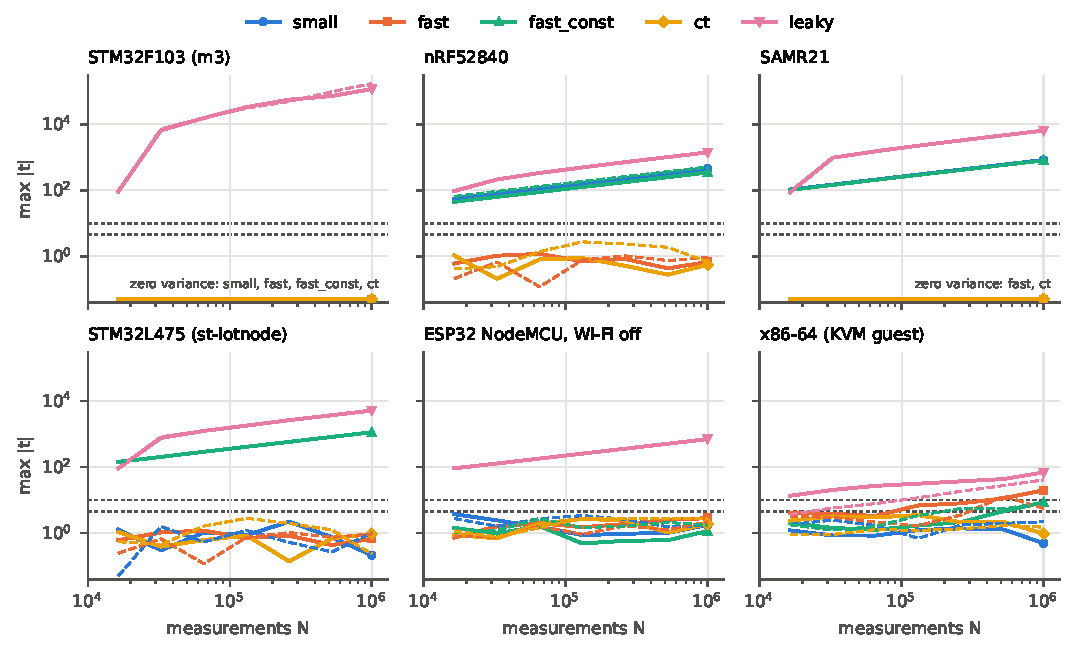
\includegraphics[width=\textwidth]{figures/paper_fig1_maxt_testA.pdf}
\caption{Maximum $|t|$ against the number of measurements, Test A. Solid lines: first run; dashed: second run (new seed, other node or core). Dotted lines: thresholds 4.5 and 10. Series with zero variance are drawn at 0.05.}
\label{fig:maxt}
\end{figure}

\textbf{Sensitivity.} \tlk{} was detected on every platform, in both tests and both runs. On the microcontrollers and ESP32 boards the mean-shift threshold of the uncropped test is about one cycle at $N=10^6$ (median 0.05--1.04, at most 2.7 cycles; Table~\ref{tab:effect}); in the placement experiment the one-iteration control \emph{lk1}, a difference of 3--7 cycles, was detected on all five microcontrollers with $|t|\geq103$. On x86-64 and the Cortex-A8 the threshold is 11--28 TSC ticks and 16--337\,ns, so small leaks there need larger $N$.

\textbf{Microcontrollers.} On the STM32F103 every real implementation took exactly the same number of cycles for all $10^6$ inputs in both runs and both tests, for example 77\,637 cycles per measurement for \tsm{} and 8\,958 for \tct{} in Test A. On the nRF52840, \tsm{} and \tfc{} leak (Test A: $|t|\geq453$ and $\geq346$), and in Test B so does \tfa{} through its key schedule, while \tfa{} in Test A and \tct{} do not. On the SAMR21 every implementation that reads a table in flash leaks ($|t|$ between 725 and 868 for the smaller run), while \tfa{} in Test A and \tct{} are constant. On the STM32L475 only \tfc{} leaks ($|t|\geq1078$); the 16-byte \texttt{S} of \tsm{} does not. On the RP2040 only \tfc{} leaks, weakly but repeatedly ($|t|\geq10.1$ and $\geq6.2$). In cycles these leaks are small: the mean differences are $+8.8$ cycles for \tsm{} on the nRF52840, $-6.0$ and $-9.5$ for \tsm{} and \tfc{} on the SAMR21, $+20.5$ for \tfc{} on the STM32L475 and $+4.7$ on the RP2040, out of 15\,000--80\,000 cycles per block. They are statistically unambiguous because the timing noise on these boards is a few cycles.

\textbf{ESP32 family.} No implementation other than \tlk{} crossed 4.5 on the ESP32, the ESP32-C6 or the second ESP32 board, also with the Wi-Fi radio scanning continuously on the other core, and the mean-shift threshold is about one cycle. A plausible explanation is that the 2.5\,KB of tables stay in the 32\,KB flash cache after the first access; we did not measure the cache state, so this is a hypothesis, and ``no leak found at $10^6$'' is the result. The timing is not exactly constant (for \tsm{} it varies by up to 4 cycles), but the variation does not separate the classes. With interrupts disabled the cycle counts are a deterministic function of the input: the two ESP32 boards, of silicon revisions 1 and 3, returned identical cycle counts for identical input sequences.

\textbf{CPU data caches.} On x86-64, \tfa{} and \tfc{} leak in Test A ($|t|\geq5.6$ and $\geq8.3$ at $N=10^6$; $\geq8.1$ and $\geq9.2$ in two further runs at $N=10^7$), and \tfa{} also in Test B at $N=10^7$. \tsm{}, whose 16-byte table lies in one cache line, and \tct{} show no leak at $N=10^7$ ($|t|\leq2.1$). On the Cortex-A8 nothing except \tlk{} leaks at $N=10^6$. At $N=10^7$, \tfc{} leaks in both tests ($|t|\geq6.7$ and $\geq9.6$), while \tfa{}, with the same tables and code in a different memory section, does not. Both copies are in RAM; they differ in their addresses, which may give different set conflicts in the 16\,KB L1 data cache, but this was not tested.

\subsection{Controlled placement experiment}

Tables~\ref{tab:placement} and~\ref{tab:placementB} show the controlled experiment: 14 runs on 14 nodes of five microcontroller types, 168 series, all of which match the host recomputation exactly. Since the code is identical, any difference between a flash and a RAM column is caused by the table address alone.

\begin{table}[!htbp]
\centering
\caption{Controlled placement experiment, Test A (fixed vs random plaintext): identical code, tables read from flash (fl) or RAM. S: 16-byte S-box of \tsm{} (aligned to 64 bytes); T: tables of \tfa{} plus the S-box; lk1, lk32: positive controls with 1 and 32 dummy iterations. Cells as in Table~\ref{tab:results}; in brackets, for repeated leaks, the mean difference random $-$ fixed in cycles (average of the two runs). $N=10^6$ per run, two nodes per row.}
\label{tab:placement}
\footnotesize
\resizebox{\textwidth}{!}{\begin{tabular}{llrrrrrr}
\hline
Platform & Setting & S fl & S ram & T fl & T ram & lk1 & lk32\\
\hline
STM32F103 & none & $=$ & $=$ & $=$ & $=$ & \textbf{116\,790} {\scriptsize(+3.0)} & \textbf{85\,915} {\scriptsize(+160.2)}\\
nRF52840 & I-cache on (default) & 0.3 & 0.5 & \textbf{848} {\scriptsize(-6.0)} & 0.3 & \textbf{620} {\scriptsize(+4.5)} & \textbf{29\,003} {\scriptsize(+128.0)}\\
nRF52840 & I-cache off & $=$ & $=$ & \textbf{492} {\scriptsize(+1.3)} & $=$ & \textbf{112\,067} {\scriptsize(+3.5)} & \textbf{102\,502} {\scriptsize(+173.3)}\\
nRF52840 & cipher code in RAM & 0.9 & 0.8 & \textbf{850} {\scriptsize(-6.4)} & 1.1 & \textbf{4\,592} {\scriptsize(+6.0)} & \textbf{96\,122} {\scriptsize(+160.4)}\\
SAMR21 & NVM cache 64\,B & \textbf{1\,018} {\scriptsize(+10.0)} & $=$ & \textbf{680} {\scriptsize(+13.0)} & $=$ & \textbf{112\,737} {\scriptsize(+7.0)} & \textbf{91\,419} {\scriptsize(+146.2)}\\
STM32L475 & ART D-cache 256\,B & 0.5 & 0.7 & \textbf{1\,130} {\scriptsize(+20.5)} & 0.3 & \textbf{276} {\scriptsize(+4.4)} & \textbf{5\,203} {\scriptsize(+127.9)}\\
RP2040 & XIP cache 16\,KB & 0.9 & 0.6 & \textbf{10.4} {\scriptsize(+10.4)} & 0.8 & \textbf{115} {\scriptsize(+5.4)} & \textbf{685} {\scriptsize(+144.3)}\\
\hline
\end{tabular}
}
\end{table}

\begin{table}[!htbp]
\centering
\caption{Controlled placement experiment, Test B (fixed vs random key, key schedule timed); columns as in Table~\ref{tab:placement}.}
\label{tab:placementB}
\footnotesize
\resizebox{\textwidth}{!}{\begin{tabular}{llrrrrrr}
\hline
Platform & Setting & S fl & S ram & T fl & T ram & lk1 & lk32\\
\hline
STM32F103 & none & $=$ & $=$ & $=$ & $=$ & \textbf{132\,885} {\scriptsize(+3.0)} & \textbf{112\,265} {\scriptsize(+160.7)}\\
nRF52840 & I-cache on (default) & 1.0 & 0.6 & \textbf{845} {\scriptsize(-6.1)} & 0.4 & \textbf{706} {\scriptsize(+4.5)} & \textbf{9\,450} {\scriptsize(+128.2)}\\
nRF52840 & I-cache off & $=$ & $=$ & \textbf{492} {\scriptsize(+1.3)} & $=$ & \textbf{176\,619} {\scriptsize(+3.5)} & \textbf{95\,205} {\scriptsize(+173.6)}\\
nRF52840 & cipher code in RAM & 0.1 & 0.7 & \textbf{845} {\scriptsize(-6.4)} & 0.5 & \textbf{1\,689} {\scriptsize(+6.0)} & \textbf{66\,855} {\scriptsize(+160.6)}\\
SAMR21 & NVM cache 64\,B & \textbf{1\,019} {\scriptsize(+10.0)} & $=$ & \textbf{703} {\scriptsize(+12.9)} & $=$ & \textbf{99\,868} {\scriptsize(+7.0)} & \textbf{138\,048} {\scriptsize(+146.7)}\\
STM32L475 & ART D-cache 256\,B & 0.3 & 0.6 & \textbf{1\,146} {\scriptsize(+20.8)} & 0.5 & \textbf{705} {\scriptsize(+4.4)} & \textbf{2\,542} {\scriptsize(+128.2)}\\
RP2040 & XIP cache 16\,KB & 0.4 & 0.4 & \textbf{9.5} {\scriptsize(+10.4)} & 0.1 & \textbf{103} {\scriptsize(+5.4)} & \textbf{682} {\scriptsize(+145.1)}\\
\hline
\end{tabular}
}
\end{table}

On every board, every RAM column is clean or constant: on the STM32F103 all four variants are constant, and the SAMR21 and the nRF52840 with disabled instruction cache are constant for both RAM variants. This includes the key schedule, which now also reads its S-box from RAM; in the main experiment the flash S-box of the key schedule was the reason why \tfa{} leaked in Test B. The flash columns leak on four boards. The large tables (T fl) leak on the nRF52840, the SAMR21, the STM32L475 and, weakly, the RP2040; the 16-byte S-box (S fl) leaks only on the SAMR21. On the nRF52840, the aligned S-box no longer leaks ($|t|\leq1.0$), whereas the S-box of \tsm{} in the main experiment did. On the nRF52840 the verdicts are the same with the instruction cache disabled and with the cipher code in RAM, so the instruction cache is not necessary for the leak. The size and sign of the mean difference do change (T fl, Test A: $-6.0$, $+1.3$ and $-6.4$ cycles), so instruction fetches still influence the timing.

\subsection{Flash read blocks}

Table~\ref{tab:mb} gives the lookup latency. On the STM32F103 a pair of flash loads always takes 11 cycles, whatever the addresses, which matches the constant timing above. On the nRF52840 the second load takes 3 cycles less when it falls into the same aligned 16-byte block as the first; the result is identical with the instruction cache disabled and in the build with the cipher code in RAM (where the microbenchmark itself still runs from flash), and RAM loads always take 5 cycles. This 16-byte block-dependent flash-read timing is consistent with a data read buffer between the core and the flash, which the product specification does not document for data reads \citep{nrf52840}; the measurement does not identify the hardware structure itself. On the SAMR21 and the STM32L475 the corresponding block is 8 bytes, matching the 64-bit lines of the SAMR21 NVM cache \citep{samr21}. On the RP2040 the reset sequence does not evict the 16\,KB XIP cache, so the microbenchmark sees only hits and does not identify the mechanism of its leak; the placement experiment shows only that the leak requires the tables in flash.

\begin{table}[!htbp]
\centering
\caption{Lookup microbenchmark: time of two consecutive byte loads (cycles, including timer overhead) when the second address lies in the same aligned block as the first or in another block; the microbenchmark code runs from flash in all builds; identical on both nodes of every type; where a block was found, the 32$\times$32 address-pair matrix agreed with it in all 1\,024 cells.}
\label{tab:mb}
\footnotesize
\begin{tabular}{llrrrrr}
\hline
Platform & Setting & \multicolumn{3}{c}{Flash: pair latency (cycles)} & RAM & \\
 & & same block & other block & block size & & \\
\hline
STM32F103 & none & 11 & 11 & -- & 9 & \\
nRF52840 & I-cache on (default) & 8 & 11 & 16\,B & 5 & \\
nRF52840 & I-cache off & 8 & 11 & 16\,B & 5 & \\
nRF52840 & cipher code in RAM & 8 & 11 & 16\,B & 5 & \\
SAMR21 & NVM cache 64\,B & 10 & 12 & 8\,B & 9 & \\
STM32L475 & ART D-cache 256\,B & 9 & 13 & 8\,B & 5 & \\
RP2040 & XIP cache 16\,KB & 8 & 8 & -- & 8 & \\
\hline
\end{tabular}

\end{table}

On the nRF52840, the SAMR21 and the STM32L475 these blocks are consistent with the leaks of the survey. A lookup leaks when the secret index decides whether consecutive reads hit the same block, and this depends on table size, block size and alignment. In the nRF52840 build of the main experiment, the 16-byte S-box of \tsm{} started at address \texttt{0x63D8}, eight bytes into a 16-byte block, so indices 0--7 and 8--15 fell into two blocks; aligned, it fits into one block and does not leak. On the SAMR21 the blocks are 8 bytes, so any 16-byte table spans two of them and leaks from flash. On the STM32L475 the 256-byte data cache holds the S-box during an encryption, while the 2.5\,KB of tables do not fit. The STM32F103 has no such block for data and is constant.

\subsection{Cost}

Table~\ref{tab:cost} and Figure~\ref{fig:cost} give the cost. With precomputed round keys, \tct{} encrypts a block in 0.11--0.17 of the time of \tsm{} on the microcontrollers and in 0.29 on x86-64, and it is also faster than \tfa{}. The bitsliced S-box handles all 16 nibbles at once, and the permutation takes 25 mask-and-shift steps instead of 64 single-bit steps. Its key schedule is 2.0--2.6 times slower than that of \tsm{}, because each of the three S-box applications per round evaluates the full formula; if a new key is expanded for every block, \tct{} is 2.2--6.2 times faster than \tsm{} (2.2 on x86-64). Its code is about twice as large (1.1--1.5\,KB), but it needs no table: \tfa{} needs 5.2\,KB of RAM for its tables, and \tfc{} 2.6\,KB of flash.

\begin{table}[!htbp]
\centering
\caption{Cost: median over 9 runs of 64 chained blocks, per block. Code: encryption plus 128-bit key schedule in the linked build. $^{\dagger}$Nanoseconds (no cycle counter). $^{\ddagger}$TSC ticks. The second ESP32 board gives the same cycle counts as the first.}
\label{tab:cost}
\footnotesize
\resizebox{\textwidth}{!}{\begin{tabular}{lrrrrrrrr}
\hline
 & \multicolumn{4}{c}{Encryption, cycles/block} & & \multicolumn{2}{c}{Key schedule} & \\
Platform & small & fast & fast\_const & ct & ct/small & small & ct & code small/ct (B)\\
\hline
STM32F103 (M3) & 77616 & 21209 & 26223 & 8937 & 0.12 & 2284 & 4455 & 520 / 1110\\
nRF52840 (M4F) & 54577 & 15202 & 17264 & 6531 & 0.12 & 1636 & 3264 & 520 / 1140\\
SAMR21 (M0+) & 80247 & 21199 & 22606 & 13527 & 0.17 & 3120 & 8032 & 596 / 1260\\
STM32L475 (M4F) & 53772 & 15196 & 17826 & 5694 & 0.11 & 1534 & 3266 & 520 / 1140\\
RP2040 (M0+) & 73613 & 20176 & 20164 & 10356 & 0.14 & 2522 & 6664 & 596 / 1260\\
ESP32 NodeMCU & 57532 & 18543 & 18560 & 6180 & 0.11 & 1967 & 4368 & 506 / 1075\\
ESP32-C6 & 49402 & 15480 & 16052 & 5992 & 0.12 & 1727 & 3381 & 628 / 1422\\
Cortex-A8 (Linux)$^{\dagger}$ & 44668 & 17306 & 17179 & 5018 & 0.11 & 1355 & 3322 & 608 / 1496\\
x86-64 (KVM)$^{\ddagger}$ & 4821 & 1809 & 1908 & 1388 & 0.29 & 391 & 1003 & 534 / 1365\\
\hline
\end{tabular}
}
\end{table}

\begin{figure}[!htbp]
\centering
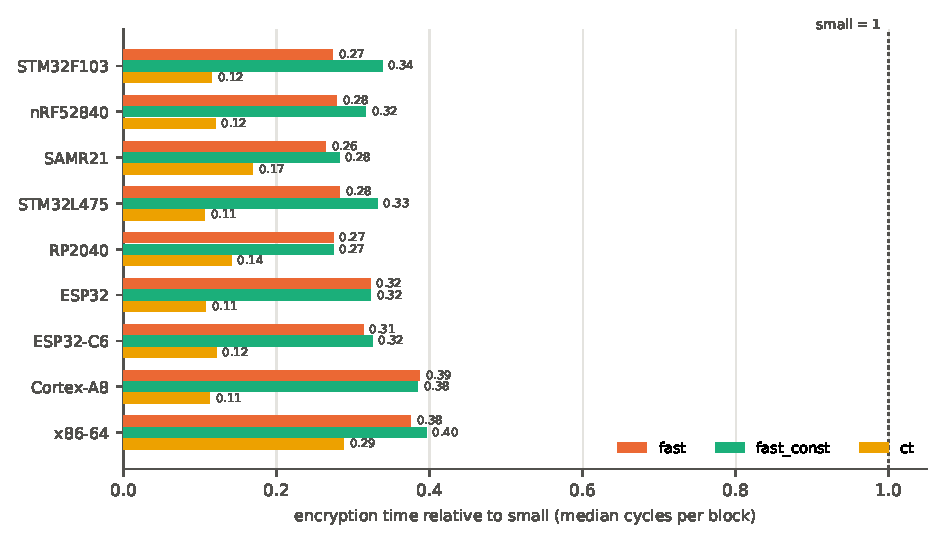
\includegraphics[width=0.9\textwidth]{figures/paper_fig2_cost.pdf}
\caption{Encryption time of \tfa{}, \tfc{} and \tct{} relative to \tsm{} on the same platform (median cycles per block with precomputed round keys; ns on the Cortex-A8, TSC ticks on x86-64). The second ESP32 board and the runs with Wi-Fi load give the same values as the ESP32 shown.}
\label{fig:cost}
\end{figure}

%=====================================================================
\section{Discussion}

The common assumption that a table lookup on a microcontroller without a data cache takes constant time holds exactly on the STM32F103, but not in general. The controlled experiment shows that on the nRF52840, the SAMR21, the STM32L475 and the RP2040 the location of a table decides: the same code with the same tables leaks from flash and is clean, often exactly constant, from RAM. For three of the boards the microbenchmark shows why: their flash reads have 8- or 16-byte blocks, and a secret index that selects the block becomes visible in the timing. For the RP2040 the cause was not identified. Whether a given table leaks therefore depends on its size and alignment relative to the block, which is why a 16-byte S-box leaked on the nRF52840 in one build and not in another. Two practical consequences follow. First, declaring a secret-indexed table \texttt{const} places it in flash with standard toolchains and can create a leak; copying it to RAM removed the leak on all five boards tested. Second, a rule such as ``the table fits into one cache line'' is fragile, because it depends on undocumented block sizes and on the address chosen by the linker.

The differences are small in cycles: a few cycles per encryption out of tens of thousands. Whether they are exploitable depends on how precisely an attacker can time the device, which we did not study. They are, however, systematic and clearly measurable, and they come from the same kind of secret-dependent memory access that cache attacks exploit on larger processors.

For Dipper itself the recommendation is to use the bitsliced implementation. It showed no leak on any platform, has no secret-dependent branches or addresses in six instruction sets, needs no tables, and is faster than both table-based profiles. This agrees with the experience with bitsliced and fixsliced GIFT \citep{adomnicai2020}. The contribution of this work is therefore not a new cipher or statistical method, but cross-device measurements with a repetition rule, a controlled separation of table placement from code, and an explanation of the observed leaks.

\textbf{Limitations.}
\begin{itemize}
\item The x86-64 platform is a virtual machine on a shared server, so its noise level is higher than on bare metal, and leaks there appear only at larger $N$.
\item On the Cortex-A8 the timer has 77\,ns steps and a system-call overhead; the \tfc{} leak there was not explained.
\item The ESP32 boards were not included in the controlled placement experiment, and their cache state was not measured. The leak on the RP2040 was not explained by the microbenchmark.
\item The mean-shift threshold is not a detection power and assumes stable variances over a run.
\item The tests cover first- and second-order differences of the timing distributions and do not include key-recovery attacks.
\item The host recomputation covers the first 131\,072 samples of each run; on the ESP32 serial links 18 of the 260 raw dumps of the main experiment were damaged and could not be compared.
\item ``No leak found'' holds for the stated $N$ and is not a proof of constant time.
\end{itemize}

%=====================================================================
\section{Conclusion}

We assessed five C implementations of the Dipper lightweight block cipher for timing leakage on ten hardware platforms with a common dudect-style method and a repetition rule. Table lookups leaked where the memory path between core and table has a block structure that the secret index can select: from flash on four of five microcontrollers, but not from RAM, and for large tables on x86-64 and the Cortex-A8. A controlled experiment with identical code showed that table placement alone decides on these boards, and a lookup microbenchmark traced the leaks on three of them to flash read blocks of 8 or 16 bytes, among them a 16-byte block effect on the nRF52840 that is consistent with an undocumented flash data read buffer. A bitsliced constant-time implementation leaked on no platform, passed static checks on six instruction sets, and was the fastest variant everywhere. The code, the firmware, the raw measurements and the scripts that produce every number in this paper are available at \url{https://github.com/AlexGuseinov/dipper-timing}.

\section{Acknowledgement}
Experiments on the Cortex-M, ESP32 and Cortex-A8 boards were carried out on the FIT IoT-LAB testbed.

\bigskip

\begin{thebibliography}{99}

\bibitem[\protect\citeauthoryear{Adjih et al.}{2015}]{adjih2015}
Adjih, C., Baccelli, E., Fleury, E., Harter, G., Mitton, N., Noel, T., Pissard-Gibollet, R., Saint-Marcel, F., Schreiner, G., Vandaele, J. \& Watteyne, T. (2015). FIT IoT-LAB: A large scale open experimental IoT testbed. In \emph{Proceedings of the IEEE 2nd World Forum on Internet of Things (WF-IoT)} (pp. 459--464). \url{https://doi.org/10.1109/WF-IoT.2015.7389098}

\bibitem[\protect\citeauthoryear{Adomnicai et al.}{2020}]{adomnicai2020}
Adomnicai, A., Najm, Z. \& Peyrin, T. (2020). Fixslicing: A new GIFT representation -- Fast constant-time implementations of GIFT and GIFT-COFB on ARM Cortex-M. \emph{IACR Transactions on Cryptographic Hardware and Embedded Systems}, \emph{2020}(3), 402--427. \url{https://doi.org/10.46586/tches.v2020.i3.402-427}

\bibitem[\protect\citeauthoryear{Almeida et al.}{2016}]{almeida2016}
Almeida, J.B., Barbosa, M., Barthe, G., Dupressoir, F. \& Emmi, M. (2016). Verifying constant-time implementations. In \emph{Proceedings of the 25th USENIX Security Symposium} (pp. 53--70). USENIX Association.

\bibitem[\protect\citeauthoryear{Baccelli et al.}{2018}]{baccelli2018}
Baccelli, E., G\"undo\u{g}an, C., Hahm, O., Kietzmann, P., Lenders, M.S., Petersen, H., Schleiser, K., Schmidt, T.C. \& W\"ahlisch, M. (2018). RIOT: An open source operating system for low-end embedded devices in the IoT. \emph{IEEE Internet of Things Journal}, \emph{5}(6), 4428--4440. \url{https://doi.org/10.1109/JIOT.2018.2815038}

\bibitem[\protect\citeauthoryear{Banik et al.}{2017}]{banik2017}
Banik, S., Pandey, S.K., Peyrin, T., Sasaki, Y., Sim, S.M. \& Todo, Y. (2017). GIFT: A small PRESENT -- Towards reaching the limit of lightweight encryption. In \emph{Cryptographic Hardware and Embedded Systems -- CHES 2017}, LNCS 10529 (pp. 321--345). Springer. \url{https://doi.org/10.1007/978-3-319-66787-4_16}

\bibitem[\protect\citeauthoryear{Bernstein}{2005}]{bernstein2005}
Bernstein, D.J. (2005). \emph{Cache-timing attacks on AES} [Technical report]. \url{https://cr.yp.to/antiforgery/cachetiming-20050414.pdf}

\bibitem[\protect\citeauthoryear{Blackman \& Vigna}{2021}]{blackman2021}
Blackman, D. \& Vigna, S. (2021). Scrambled linear pseudorandom number generators. \emph{ACM Transactions on Mathematical Software}, \emph{47}(4), Article 36, 1--32. \url{https://doi.org/10.1145/3460772}

\bibitem[\protect\citeauthoryear{Bogdanov et al.}{2010}]{bogdanov2010}
Bogdanov, A., Eisenbarth, T., Paar, C. \& Wienecke, M. (2010). Differential cache-collision timing attacks on AES with applications to embedded CPUs. In \emph{Topics in Cryptology -- CT-RSA 2010}, LNCS 5985 (pp. 235--251). Springer. \url{https://doi.org/10.1007/978-3-642-11925-5_17}

\bibitem[\protect\citeauthoryear{Daniel et al.}{2020}]{daniel2020}
Daniel, L.-A., Bardin, S. \& Rezk, T. (2020). Binsec/Rel: Efficient relational symbolic execution for constant-time at binary-level. In \emph{Proceedings of the IEEE Symposium on Security and Privacy} (pp. 1021--1038). \url{https://doi.org/10.1109/SP40000.2020.00074}

\bibitem[\protect\citeauthoryear{Espressif Systems}{2026a}]{esp32trm}
Espressif Systems (2026a). \emph{ESP32 technical reference manual}, version 5.8. \url{https://www.espressif.com/sites/default/files/documentation/esp32_technical_reference_manual_en.pdf}

\bibitem[\protect\citeauthoryear{Espressif Systems}{2026b}]{esp32c6trm}
Espressif Systems (2026b). \emph{ESP32-C6 technical reference manual}, version 1.2. \url{https://www.espressif.com/sites/default/files/documentation/esp32-c6_technical_reference_manual_en.pdf}

\bibitem[\protect\citeauthoryear{Geimer et al.}{2023}]{geimer2023}
Geimer, A., Vergnolle, M., Recoules, F., Daniel, L.-A., Bardin, S. \& Maurice, C. (2023). A systematic evaluation of automated tools for side-channel vulnerabilities detection in cryptographic libraries. In \emph{Proceedings of the ACM SIGSAC Conference on Computer and Communications Security} (pp. 1690--1704). \url{https://doi.org/10.1145/3576915.3623112}

\bibitem[\protect\citeauthoryear{Goodwill et al.}{2011}]{goodwill2011}
Goodwill, G., Jun, B., Jaffe, J. \& Rohatgi, P. (2011). A testing methodology for side-channel resistance validation. In \emph{NIST Non-Invasive Attack Testing Workshop}. \url{https://www.rambus.com/wp-content/uploads/2015/08/a-testing-methodology-for-side-channel-resistance-validation.pdf}

\bibitem[\protect\citeauthoryear{Hansen et al.}{2020}]{hansen2020}
Hansen, A.B., Nielsen, E.H. \& Eskildsen, M. (2020). Toolchain for timing leakage analysis of NIST lightweight crypto candidates. In \emph{NIST Lightweight Cryptography Workshop 2020}. \url{https://csrc.nist.gov/CSRC/media/Events/lightweight-cryptography-workshop-2020/documents/papers/toolchain-timing-leakage-lwc2020.pdf}

\bibitem[\protect\citeauthoryear{Huseynli et al.}{2026}]{huseynli2026}
Huseynli, A., Imamverdiyev, Y. \& Alizadeh, J. (2026). Dipper: A lightweight hybrid SPN--ARX block cipher. \emph{Cryptography}, \emph{10}(4), 52. \url{https://doi.org/10.3390/cryptography10040052}

\bibitem[\protect\citeauthoryear{Jancar et al.}{2022}]{jancar2022}
Jancar, J., Fourn\'e, M., De Almeida Braga, D., Sabt, M., Schwabe, P., Barthe, G., Fouque, P.-A. \& Acar, Y. (2022). ``They're not that hard to mitigate'': What cryptographic library developers think about timing attacks. In \emph{Proceedings of the IEEE Symposium on Security and Privacy} (pp. 632--649). \url{https://doi.org/10.1109/SP46214.2022.9833713}

\bibitem[\protect\citeauthoryear{Langley}{2010}]{langley2010}
Langley, A. (2010). \emph{Checking that functions are constant time with Valgrind}. \url{https://www.imperialviolet.org/2010/04/01/ctgrind.html}

\bibitem[\protect\citeauthoryear{Lipp et al.}{2016}]{lipp2016}
Lipp, M., Gruss, D., Spreitzer, R., Maurice, C. \& Mangard, S. (2016). ARMageddon: Cache attacks on mobile devices. In \emph{Proceedings of the 25th USENIX Security Symposium} (pp. 549--564). USENIX Association.

\bibitem[\protect\citeauthoryear{Microchip Technology}{2016}]{samr21}
Microchip Technology (Atmel) (2016). \emph{SAM R21 datasheet}, Atmel-42223G.

\bibitem[\protect\citeauthoryear{Nordic Semiconductor}{2024}]{nrf52840}
Nordic Semiconductor (2024). \emph{nRF52840 product specification}, online version, section NVMC. \url{https://docs.nordicsemi.com/r/bundle/ps_nrf52840/page/nvmc.html} (accessed 20 October 2026)

\bibitem[\protect\citeauthoryear{Osvik et al.}{2006}]{osvik2006}
Osvik, D.A., Shamir, A. \& Tromer, E. (2006). Cache attacks and countermeasures: The case of AES. In \emph{Topics in Cryptology -- CT-RSA 2006}, LNCS 3860 (pp. 1--20). Springer. \url{https://doi.org/10.1007/11605805_1}

\bibitem[\protect\citeauthoryear{Raspberry Pi}{2025}]{rp2040}
Raspberry Pi Ltd (2025). \emph{RP2040 datasheet}. \url{https://datasheets.raspberrypi.com/rp2040/rp2040-datasheet.pdf}

\bibitem[\protect\citeauthoryear{Reparaz et al.}{2017}]{reparaz2017}
Reparaz, O., Balasch, J. \& Verbauwhede, I. (2017). Dude, is my code constant time? In \emph{Proceedings of Design, Automation \& Test in Europe (DATE)} (pp. 1697--1702). \url{https://doi.org/10.23919/DATE.2017.7927267}

\bibitem[\protect\citeauthoryear{Schneider \& Moradi}{2015}]{schneider2015}
Schneider, T. \& Moradi, A. (2015). Leakage assessment methodology: A clear roadmap for side-channel evaluations. In \emph{Cryptographic Hardware and Embedded Systems -- CHES 2015}, LNCS 9293 (pp. 495--513). Springer. \url{https://doi.org/10.1007/978-3-662-48324-4_25}

\bibitem[\protect\citeauthoryear{Schwabe \& Stoffelen}{2017}]{schwabe2016}
Schwabe, P. \& Stoffelen, K. (2017). All the AES you need on Cortex-M3 and M4. In \emph{Selected Areas in Cryptography -- SAC 2016}, LNCS 10532 (pp. 180--194). Springer. \url{https://doi.org/10.1007/978-3-319-69453-5_10}

\bibitem[\protect\citeauthoryear{STMicroelectronics}{2008}]{rm0008}
STMicroelectronics (2008). \emph{RM0008 reference manual: STM32F101xx--STM32F107xx}, revision 6.

\bibitem[\protect\citeauthoryear{STMicroelectronics}{2017}]{rm0351}
STMicroelectronics (2017). \emph{RM0351 reference manual: STM32L4x5 and STM32L4x6}, revision 5.

\bibitem[\protect\citeauthoryear{Texas Instruments}{2014}]{am3505}
Texas Instruments (2014). \emph{AM3517/05 Sitara ARM microprocessor datasheet}, SPRS550F.

\bibitem[\protect\citeauthoryear{Tromer et al.}{2010}]{tromer2010}
Tromer, E., Osvik, D.A. \& Shamir, A. (2010). Efficient cache attacks on AES, and countermeasures. \emph{Journal of Cryptology}, \emph{23}(1), 37--71. \url{https://doi.org/10.1007/s00145-009-9049-y}

\bibitem[\protect\citeauthoryear{Welford}{1962}]{welford1962}
Welford, B.P. (1962). Note on a method for calculating corrected sums of squares and products. \emph{Technometrics}, \emph{4}(3), 419--420. \url{https://doi.org/10.1080/00401706.1962.10490022}

\end{thebibliography}
\end{document}
